\documentclass{beamer}
\usetheme{CambridgeUS}
\usefonttheme{serif} 
\usepackage[utf8]{inputenc}
%\usepackage{default}
\usepackage{booktabs}
\usepackage{pifont}
\usepackage{lineno}
%\usepackage{beamerthemesplit}
%\usepackage{stmaryrd}
\usepackage{comment}
\usepackage{subfig}
\usepackage[percent]{overpic}
\usepackage{amsfonts}
\usepackage{amsmath}
\usepackage{amssymb}
\usepackage{movie15}
\usepackage{mathrsfs}
\usepackage{fixltx2e}
\newcommand{\argmin}[1]{\underset{#1}{\operatorname{arg}\,\operatorname{min}}\;}
\newcommand{\cmark}{\ding{51}}%
\newcommand{\xmark}{\ding{55}}%
\begin{document}

\title{Algorithms for Single Particle Reconstruction using Cryo-EM} 
\institute{Princeton University\\
\it{Joint work with Teng Zhang (UCF), Jane Zhao (UIUC) and Amit Singer (Princeton)}} 
\date{February 15, 2017} 
\author{Tejal Bhamre\\
} 
\begin{frame}
\titlepage 
\end{frame}

% 
% \begin{frame}{Overview}
% \tableofcontents
% \end{frame}
% 

\section{What is cryo electron microscopy?}

\begin{frame}<beamer>
\frametitle{Why cryo-EM?}

%  FEI
\begin{itemize}
 \item 3D structure of macromolecules - understand function 
 \item Drug discovery for cancer, AIDS, etc.
 \item X-ray crystallography: many proteins, viruses resistant to crystallization (HIV virus)
 \item Native state: can study structures impossible before!
\end{itemize}
\end{frame}

\begin{frame}<beamer>
\frametitle{Nature Method of the Year 2015}
\centering
\includegraphics[height=0.85\textheight]{nature.png}%
\end{frame}


\begin{frame}<beamer>
\frametitle{Understanding the Zika Virus}
\includegraphics[width=0.85\textwidth]{zika.png}%
\end{frame}

\begin{frame}<beamer>
\frametitle{Drug discovery for cancer}
\begin{center}
\includegraphics[width=0.95\textwidth]{cancer.png}\\\includegraphics[width=0.25\textwidth]{cancer2.png}%
\end{center}
\end{frame}

\section{Cryo-EM Pipeline}
\begin{frame}
\frametitle{3D from 2D}
%  FEI
\begin{center}
\includegraphics[width=.7\textwidth]{cryoem_image_formation.png}
\end{center}
\url{https://people.csail.mit.edu/gdp/cryoem.html}
\begin{itemize}
 \item Flash freeze sample in an ice layer
 \item Image with an electron microscope
 \item 2D images at unknown orientations $\rightarrow$ 3D structure
\end{itemize}
\end{frame}

\begin{frame}
\frametitle{3D from 2D}
%  FEI
Interdisciplinary: computer scientists/ mathematicians and biologists
\begin{center}
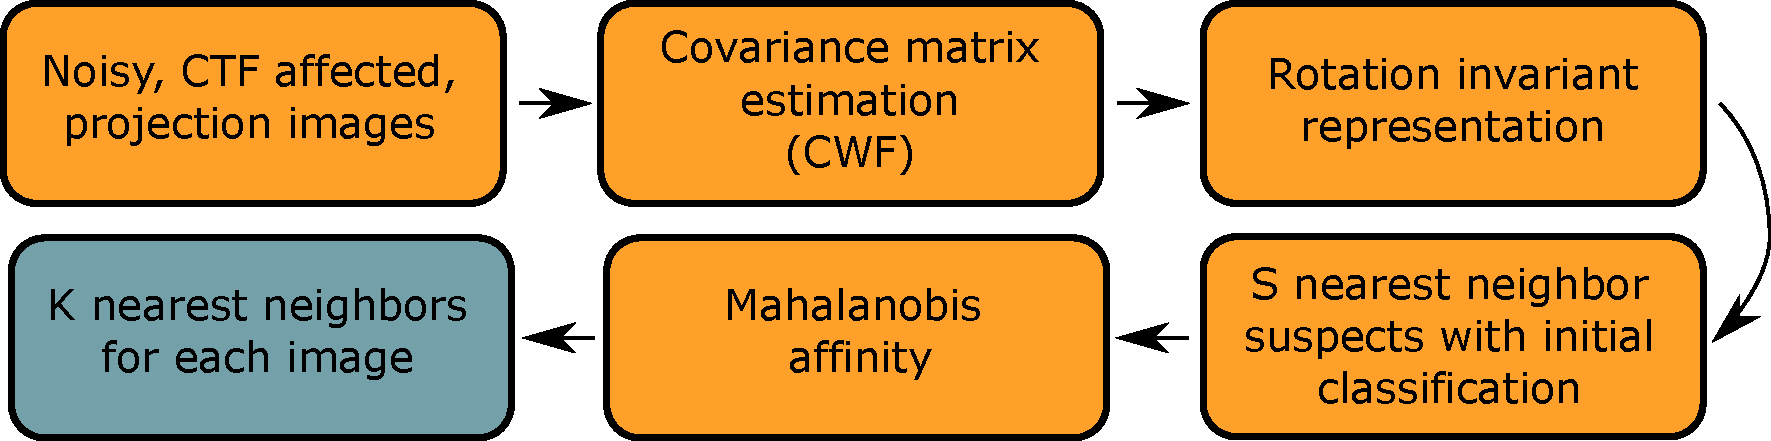
\includegraphics[width=.8\textwidth]{pipeline.png}\\
\end{center}
\small{
\url{http://goo.gl/qa6BsA},\url{http://goo.gl/Yazvxg}
}
\end{frame}

\begin{frame}
\frametitle{Image Formation}
%  FEI
Microscope filters: Contrast Transfer Function (CTF) + Noise
\begin{center}
\includegraphics[width=.85\textwidth]{cryoem_image_formation.png}
\end{center}
\url{https://people.csail.mit.edu/gdp/cryoem.html}
\end{frame}

\begin{frame}
\frametitle{Back-projection}
%  FEI
\begin{center}
\includegraphics[width=.9\textwidth]{cryoem_3d_reconstruction.png}
\end{center}
\url{https://people.csail.mit.edu/gdp/cryoem.html}\\
\vspace{5 mm}
Sounds like Structure from Motion (SfM)?
\end{frame}

\begin{frame}
\frametitle{Sounds like SfM?}
%  FEI
\begin{center}
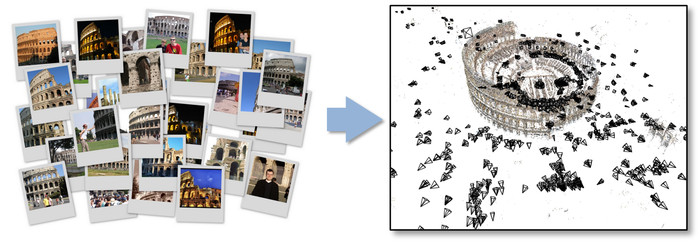
\includegraphics[width=0.8\textwidth]{bundler.jpg}%
\end{center}
\small{\url{https://www.cs.cornell.edu/~snavely/bundler/}}
\end{frame}

\begin{frame}
\frametitle{But with these images (SNR$~ 1/100$)}
%  FEI
\begin{center}
\includegraphics[width=0.8\textwidth]{raw_images.png}%
\end{center}
\begin{itemize}
  \item Can't detect features from raw images, unlike SfM
 \item Need new algorithms to handle noise level!
 \item Large number ($>100,000$) of images: 2 orders of magnitude more than SfM
\end{itemize}
\end{frame}
\begin{frame}
\frametitle{Cryo-EM Pipeline}
%  FEI
\begin{center}
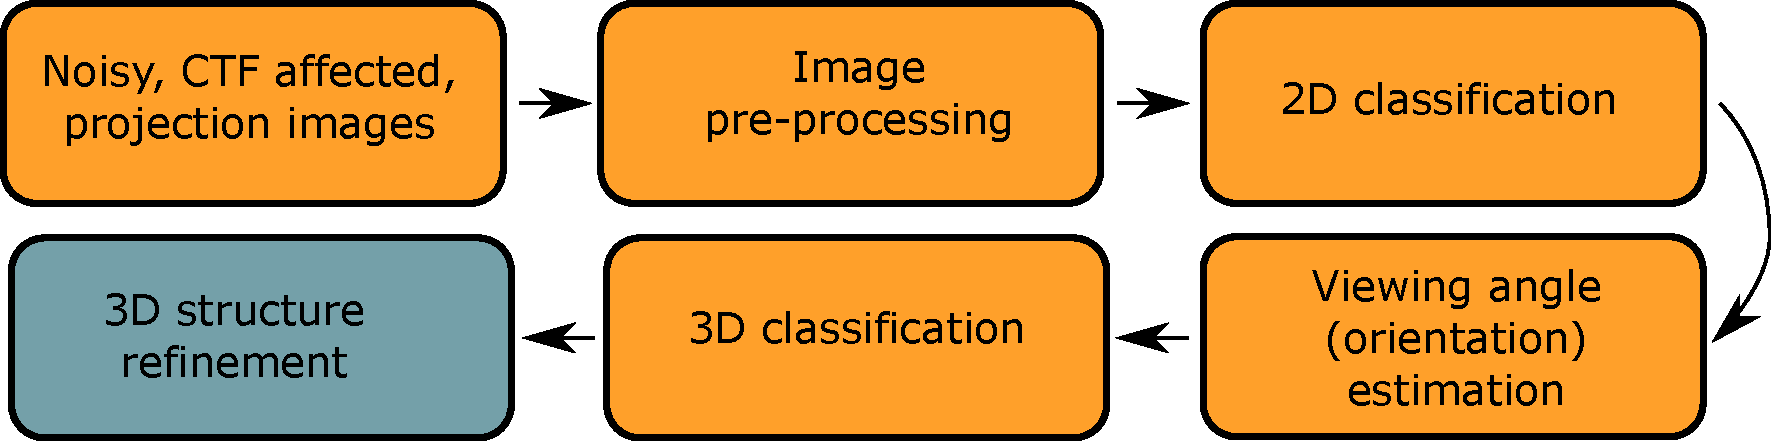
\includegraphics[width=0.9\textwidth]{cryoem_pipeline.pdf}%
\end{center}
\end{frame}

\begin{frame}
\frametitle{Open Source Software}
%  FEI
\includegraphics[width=0.9\textwidth]{Aspire.png}%
\begin{itemize}
  \item Open source software toolbox: ASPIRE
   \item \url{spr.math.princeton.edu}
   \item Improved algorithms, playground to build new ones
\end{itemize}
\end{frame}


\begin{frame}
\frametitle{Today's talk}
%  FEI
\begin{center}
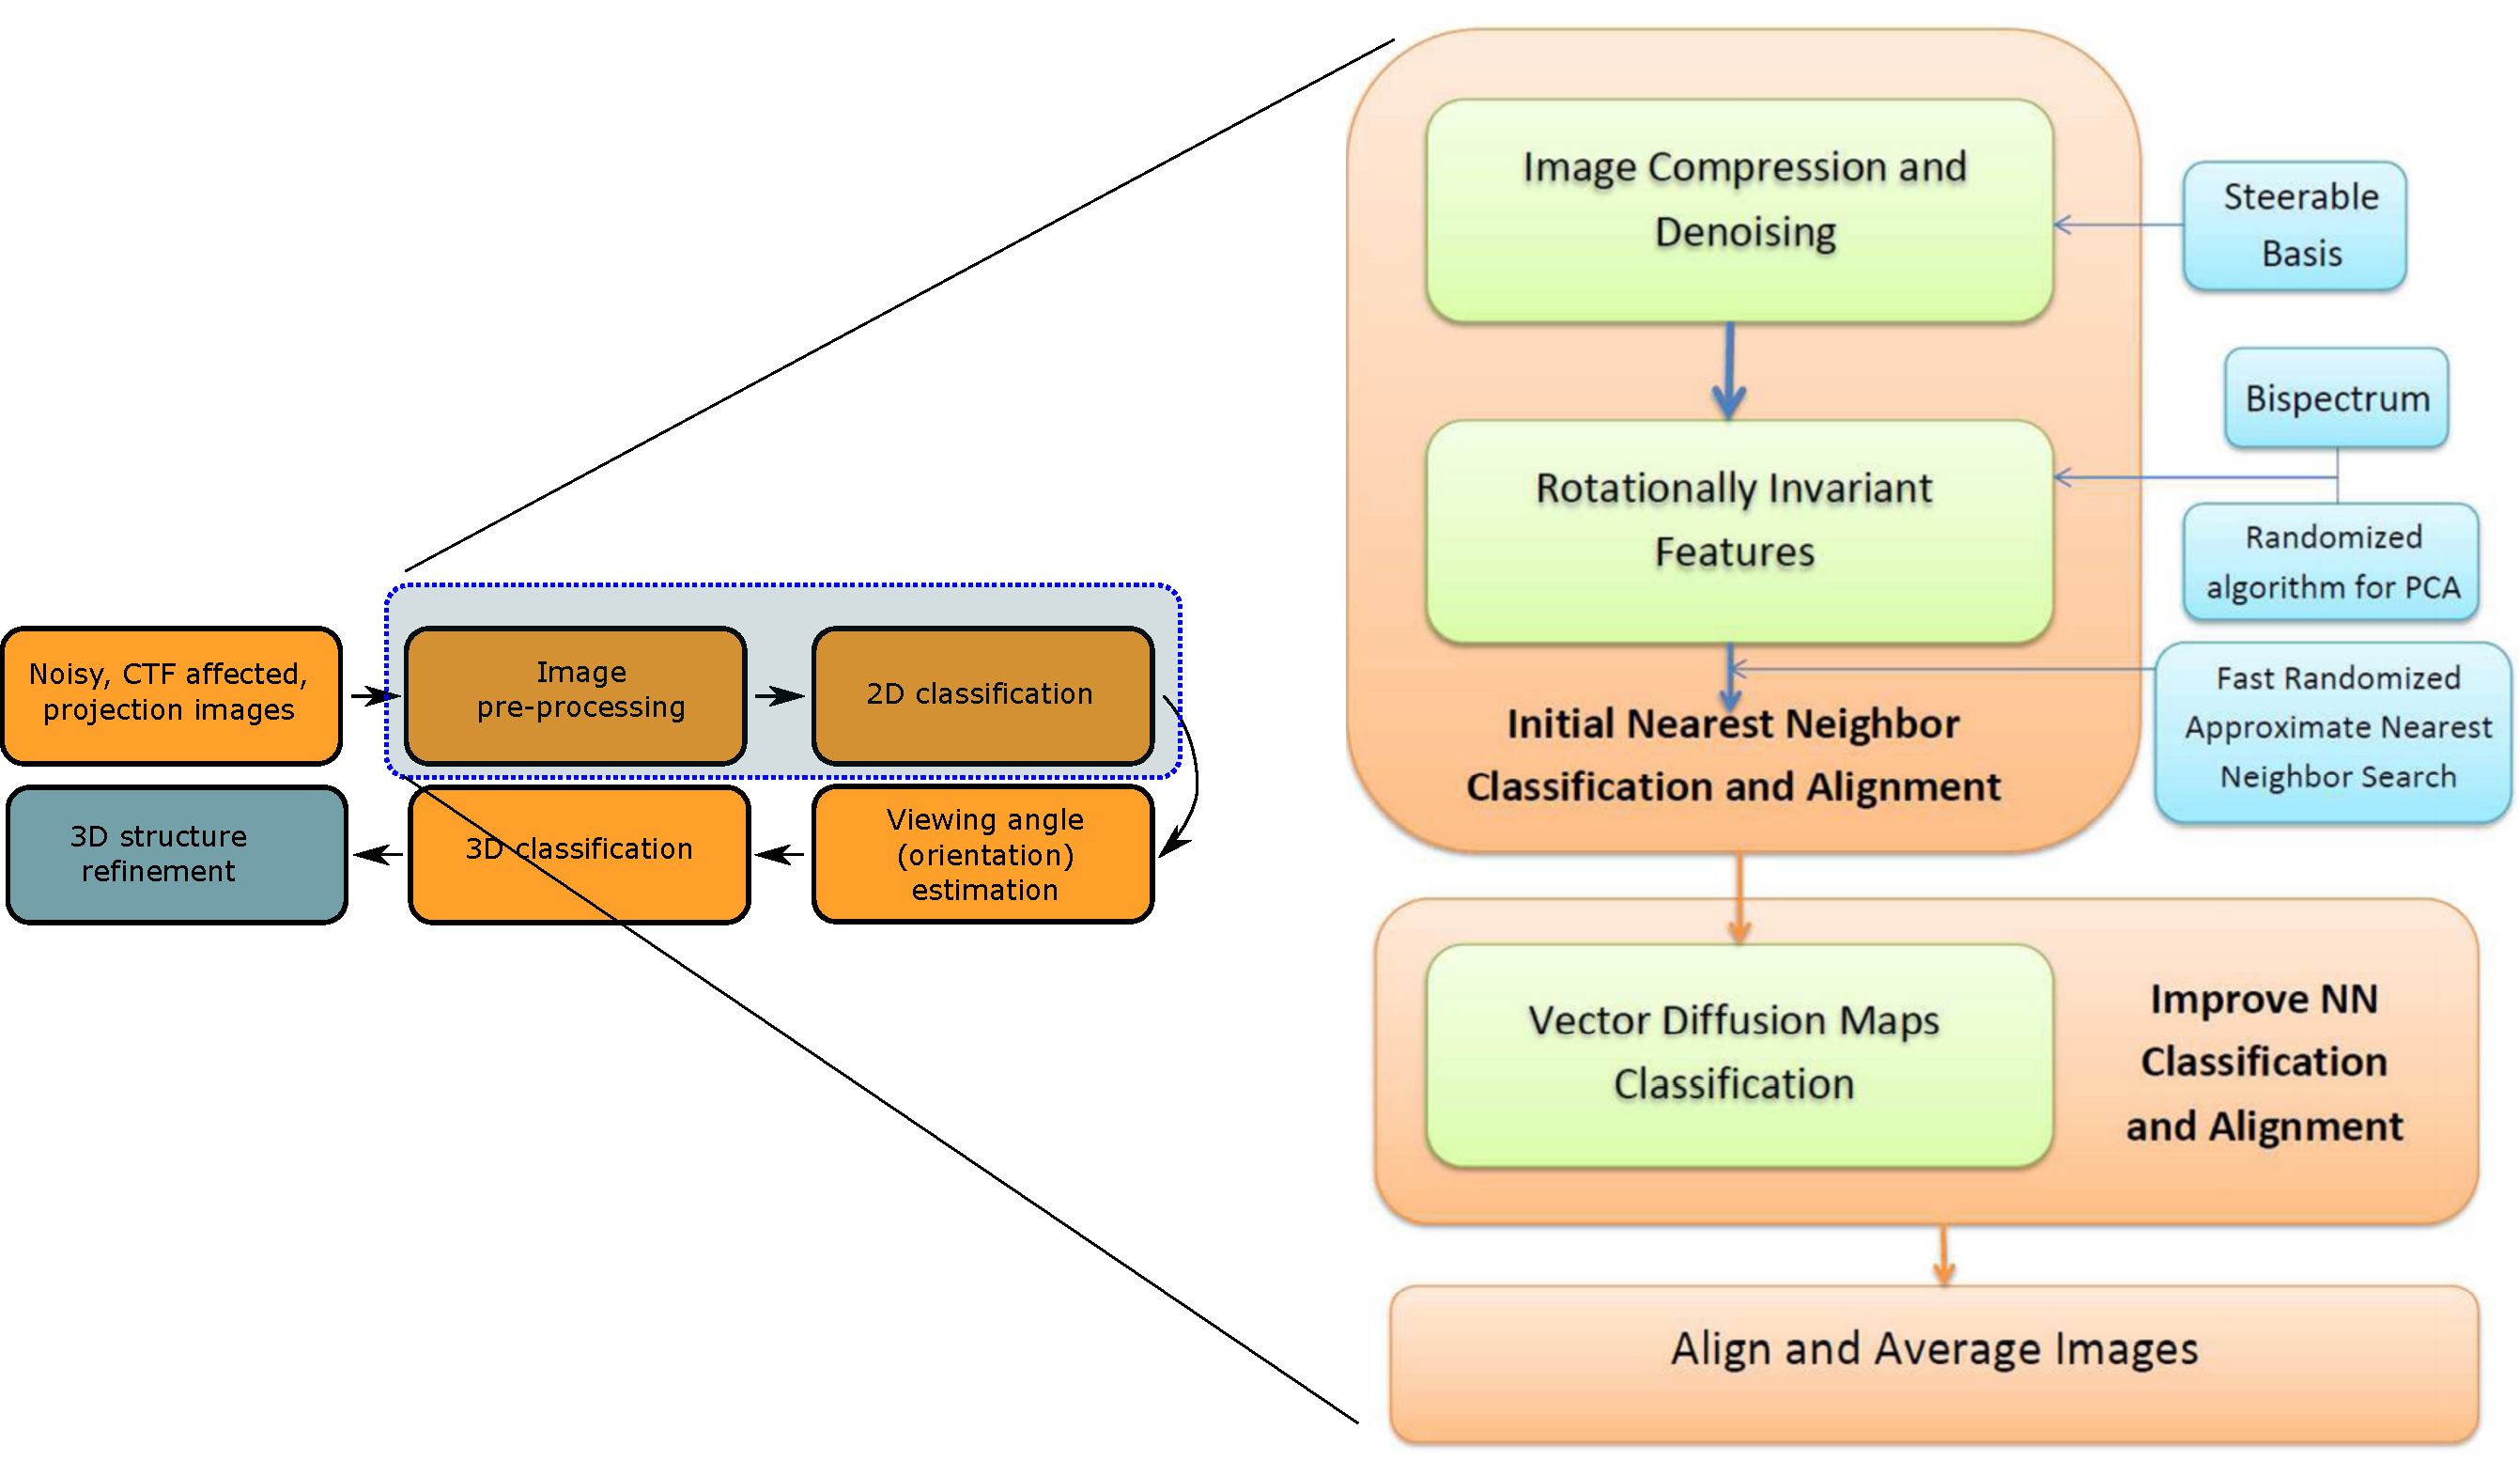
\includegraphics[width=0.9\textwidth]{cryoem_pipeline_zoom.pdf}
\end{center}

\end{frame}



\begin{frame}
\frametitle{Today's talk}
%  FEI
\begin{itemize}
{\small
\item \textit{T. Bhamre}, T. Zhang, and A. Singer ``Anisotropic Twicing: Magnitude Correction for Orthogonal Extension in Cryo-EM", in preparation (2017).
\item \textit{T. Bhamre}, Z. Zhao, and A. Singer ``Mahalanobis Distance for Class Averaging of Cryo-EM Images", 14th IEEE International Symposium on Biomedical Imaging (2017).
\item \textbf{\textit{T. Bhamre}, T. Zhang, and A. Singer ``Denoising and Covariance Estimation of Single Particle Cryo-EM Images", Journal of Structural Biology, 195 (1), pp. 72-81 (2016).}
\item \textit{T. Bhamre}, T. Zhang, and A. Singer ``Orthogonal Matrix Retrieval in Cryo-Electron Microscopy", 12th IEEE International Symposium on Biomedical Imaging, pp. 1048--1052 (2015)
\item \textit{T. Bhamre}, T. Zhang and A. Singer, ``A Semidefinite Programming Approach to 3D Reconstruction
of Macromolecules", Poster at Semidefinite Programming and Graph Algorithms, ICERM (2014)
}
\end{itemize}

\end{frame}

\section{Introduction}
\begin{frame}<beamer>
\setbeamercovered{transparent}
\frametitle{Cryo-EM Pipeline}
\begin{itemize}
 \item Particle picking from micrographs
 \item \textbf{Preprocessing}: noise estimation, prewhitening, CTF correction, denoising
 \item \textbf{2D classification (Class averaging)}: inspect underlying particles, estimate viewing angless
 \item 3D classification
 \item 3D refinement
\end{itemize}
\end{frame}

\begin{frame}<beamer>
\setbeamercovered{transparent}
\frametitle{Motivation}
\begin{itemize}
 \item Visualization of underlying particles \textbf{without class averaging} (expensive)
 \item Optimal image restoration (CTF correction and denoising) in a \textbf{single step}
  \item \textbf{Automated Outlier detection} (currently manual after averaging)
\end{itemize}
\end{frame}

\begin{frame}
\frametitle{Challenges}
%  FEI
\begin{itemize}
 \item High dimensional dataset (images $\sim 300 \times 300$ to $500 \times 500$)
 \item Very low SNR $\sim 1/100$
 \item Lost information at many frequencies
\end{itemize}
Large number of images $\sim 10^5 - 10^6$
\end{frame}

\begin{frame}<beamer>
\setbeamercovered{transparent}
\frametitle{Key novel ideas}
\begin{itemize}
 \item \textbf{Data adaptive basis}: Image compression, efficient computation (block diagonal matrix)
 \item Least squares formulation: Use information from all CTF groups to \textbf{recover lost information}
 \item Positive semidefinite matrix system: \textbf{Speed-up }
 \item Eigenvalue shrinkage: \textbf{Finite sample effect}
 \item \textbf{Asymptotically consistent estimator for covariance}
\end{itemize}
\end{frame}


\begin{frame}<beamer>
\setbeamercovered{transparent}
\frametitle{CTF Correction}
\begin{itemize}
\item CTF suppresses information and inverts contrast
\item \alert{Challenge}: CTF cannot be trivially inverted (zero crossings)
\item Information lost from one defocus group could be recovered from another group that has different zero crossings.
\end{itemize}
\vspace{-3mm}
\begin{figure}[]
%\centering
 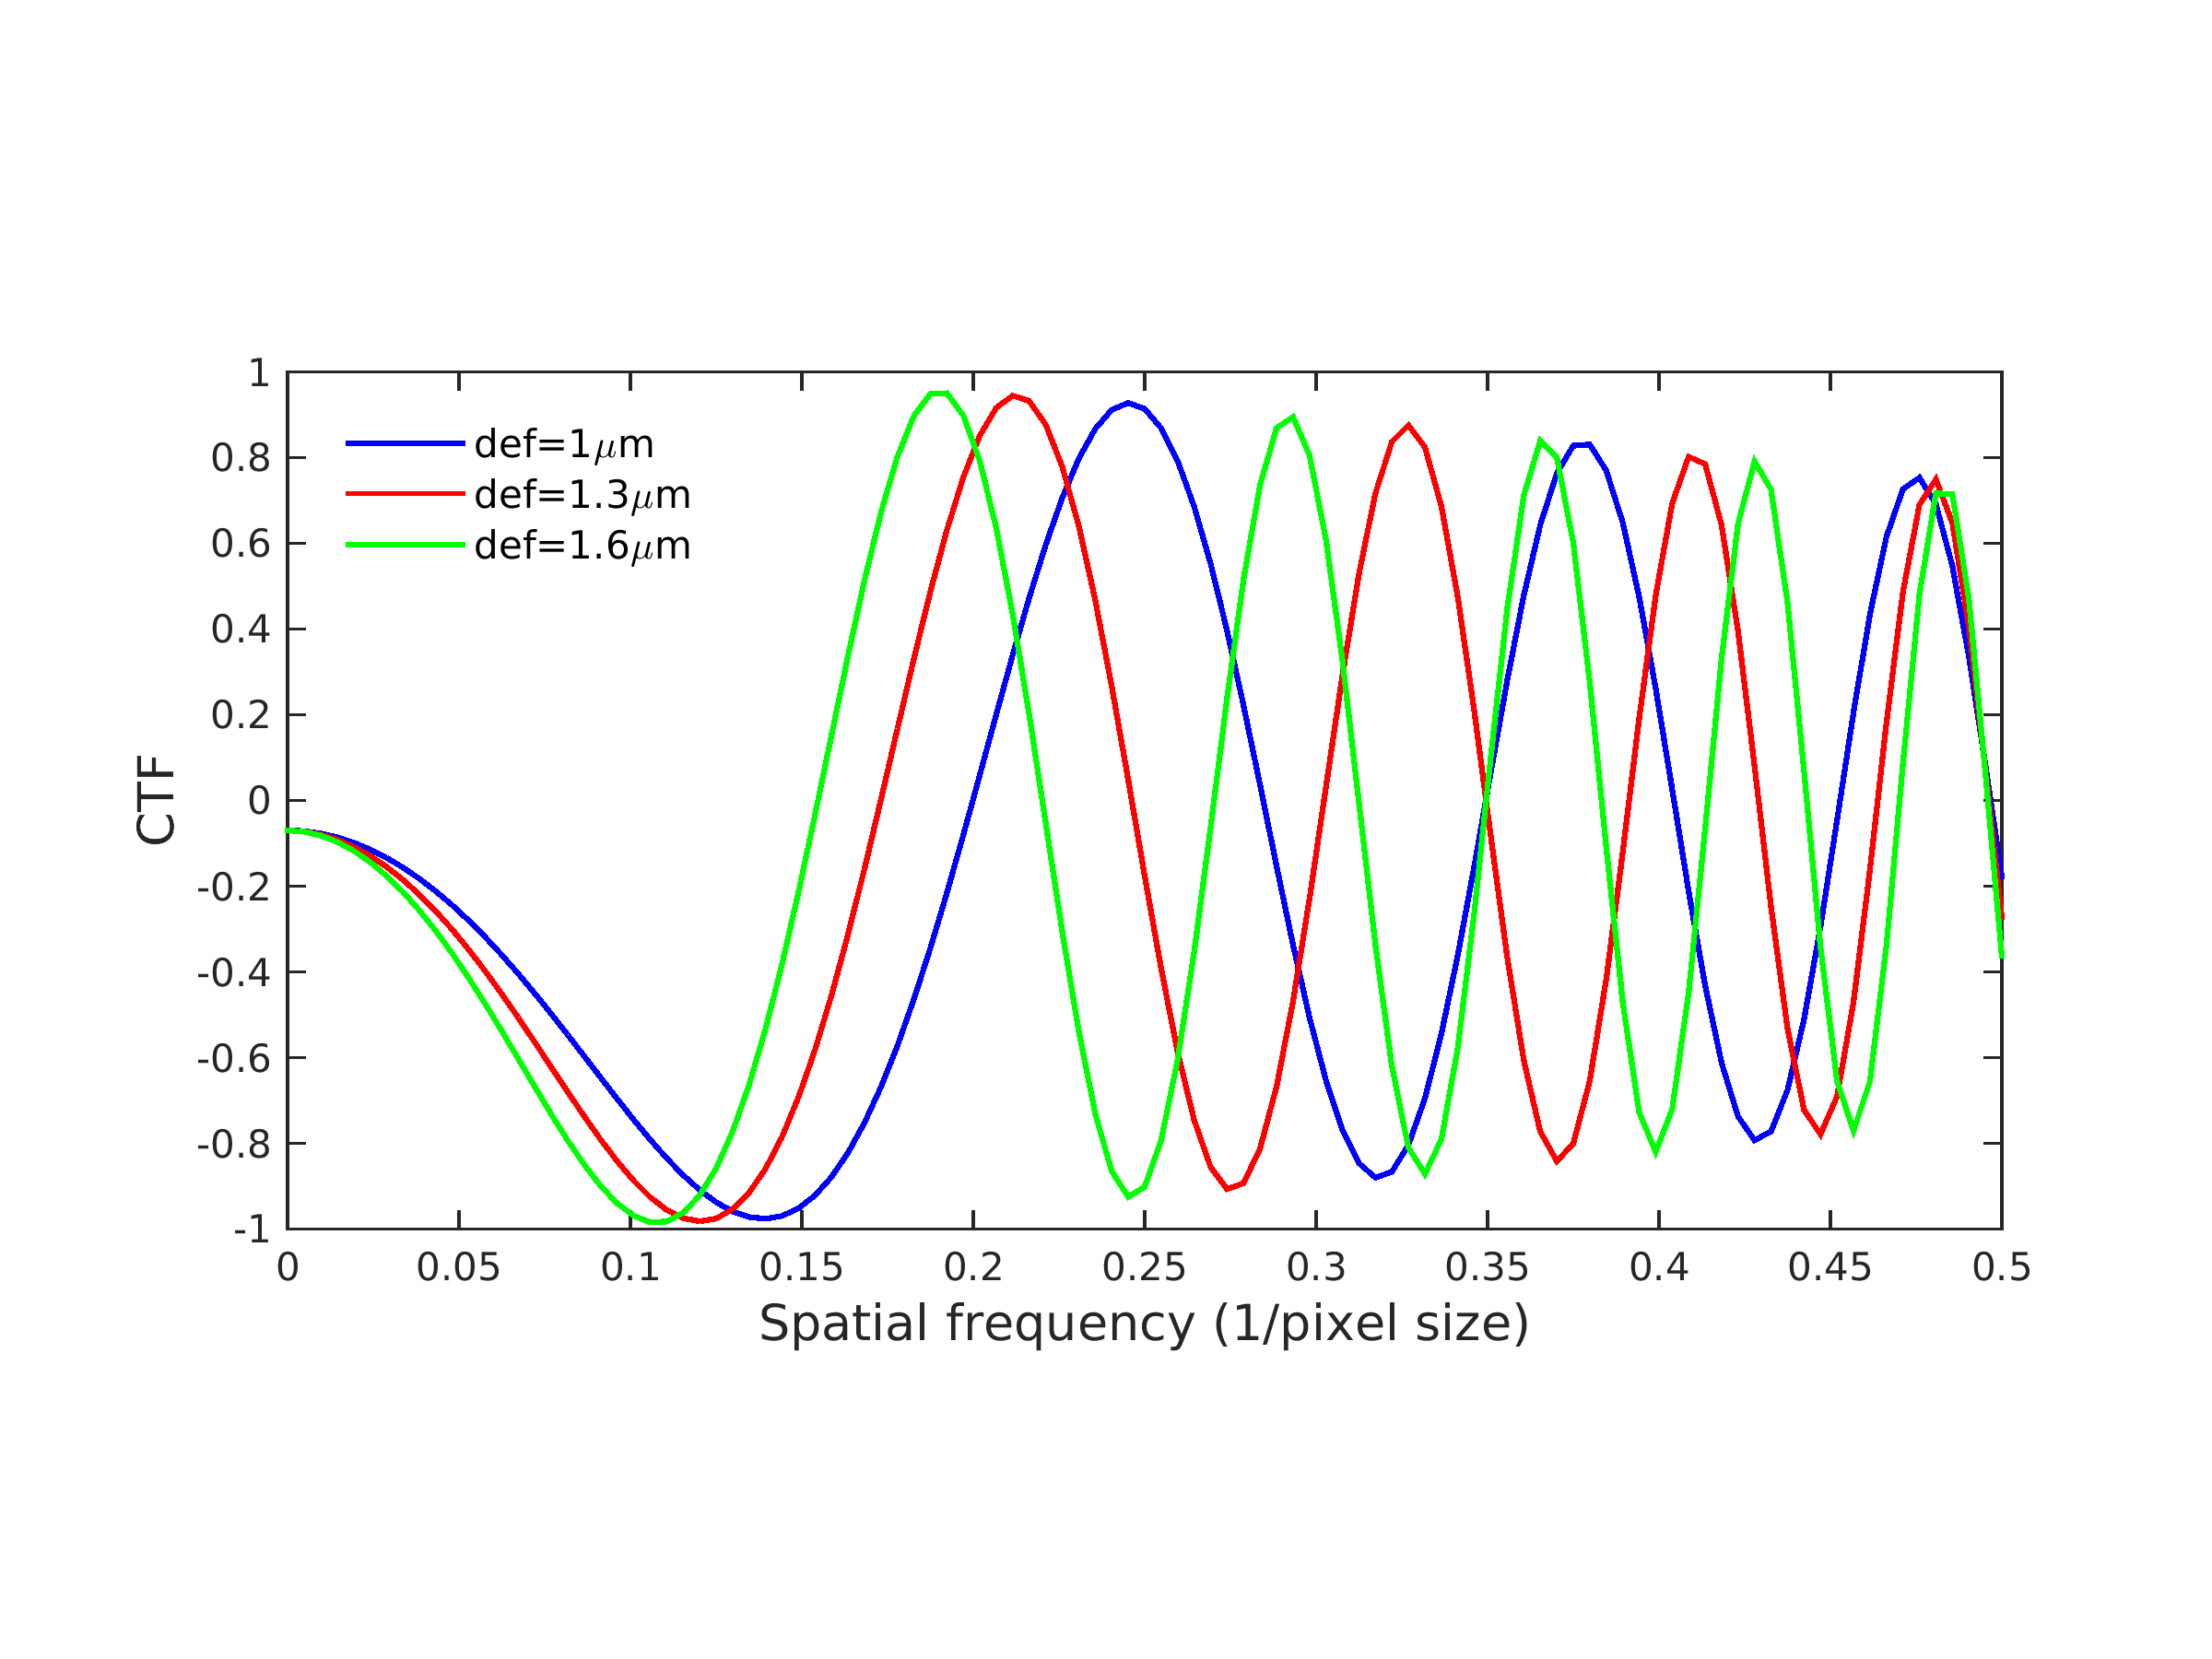
\includegraphics[scale=0.4]{ctfeg_fig.png}
 \end{figure}
 \footnote{T. Bhamre, Z. Zhao, and A. Singer ``Mahalanobis Distance for Class Averaging of Cryo-EM Images", 14th IEEE International Symposium on Biomedical Imaging (2017)}
\end{frame}


\begin{frame}<beamer>
\setbeamercovered{transparent}
\frametitle{CTF Correction}

\begin{itemize}
\item Do nothing (Denial) 
\item Correct Fourier phases but not amplitudes
\item Correct both Fourier phases and amplitudes 
\end{itemize}
\begin{figure}[]
%\centering
 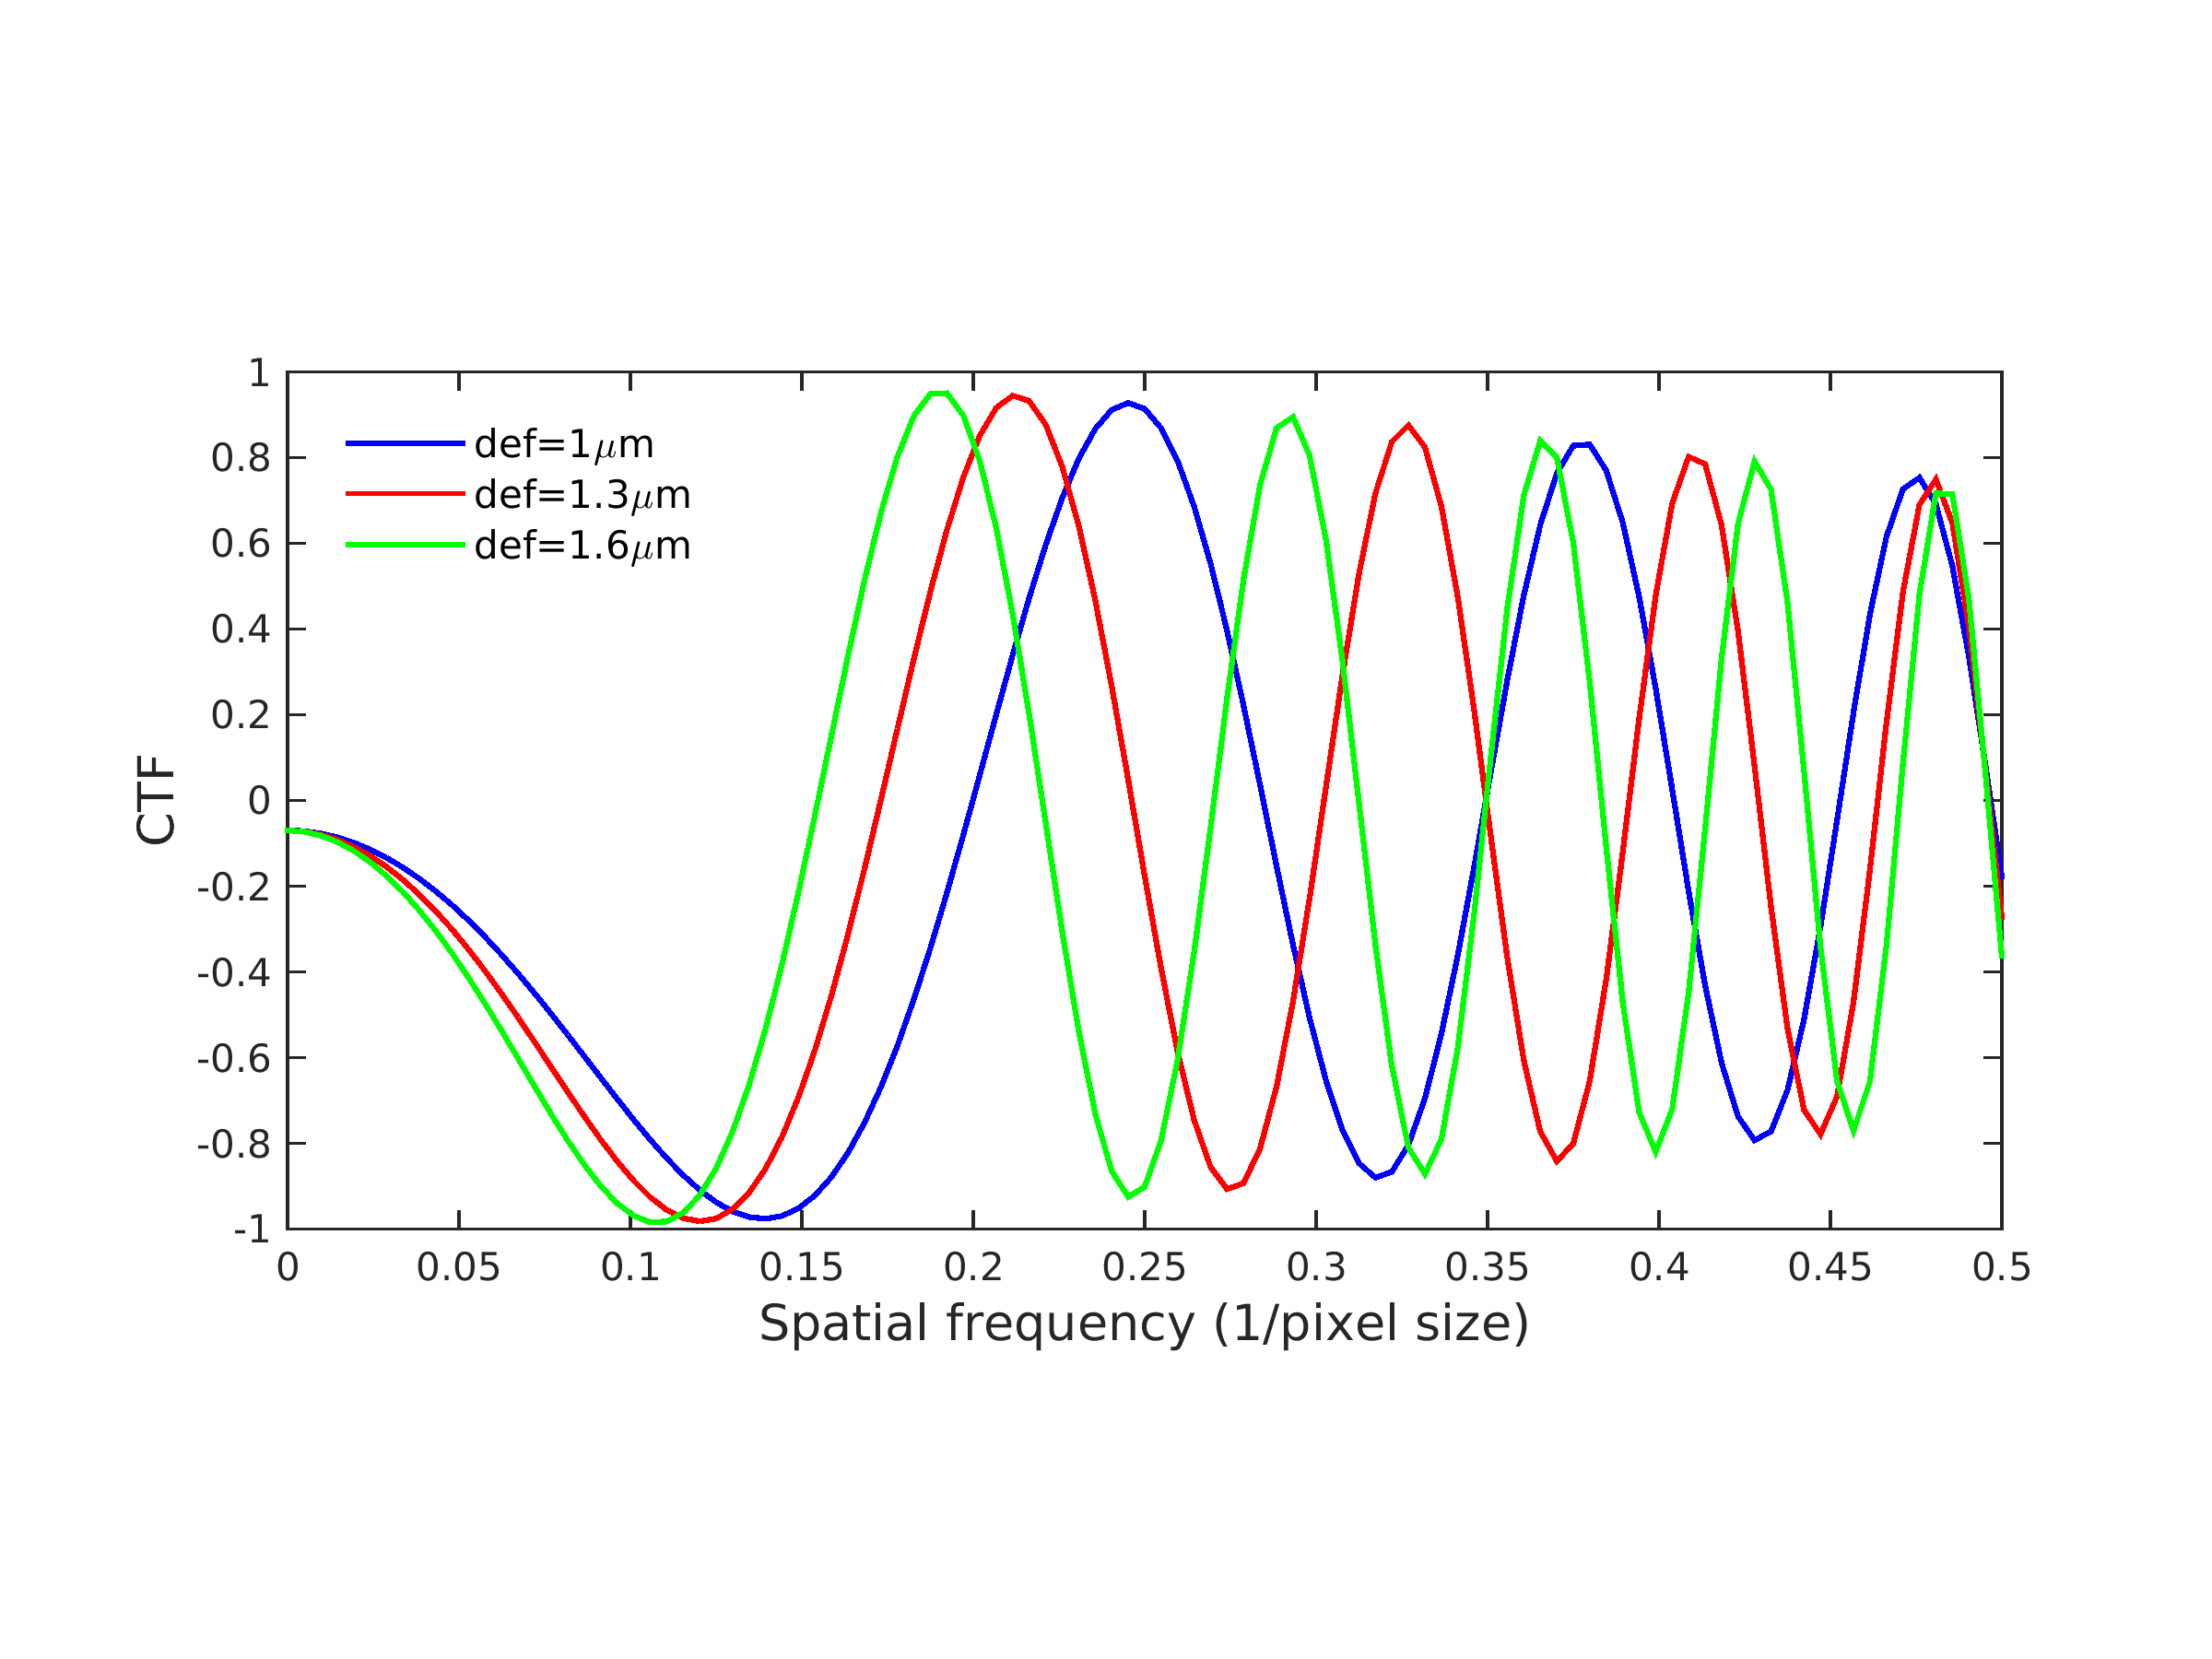
\includegraphics[scale=0.4]{ctfeg_fig.png}
 \end{figure}
\end{frame}

\begin{frame}<beamer>
\setbeamercovered{transparent}
\frametitle{Current Image Restoration Techniques}
\begin{itemize}
 \item \textbf{Phase flipping + steerable PCA (sPCA)}: 
  \begin{itemize}
  \item  Flip sign of the Fourier
coefficients at frequencies for which the CTF is negative
   \item Preserves noise statistics
   \item Data adaptive basis: eigenvectors of the sample covariance matrix
   \item Phase flipping corrects only phases
  \end{itemize}
 \item \textbf{Traditional Wiener Filtering (TWF)}:
 \begin{itemize}
  \item  Corrects both phases and amplitudes
  \item Requires prior estimation of the spectral signal to
 noise ratio (SSNR)
  \item  Cannot restore information at zero crossings of the CTF
  \item Not in a data adaptive basis (restricted to Fourier basis)
 \end{itemize}
\end{itemize}
\end{frame}


\section{Covariance Wiener Filtering (CWF)}
\begin{frame}<beamer>
\setbeamercovered{transparent}
\frametitle{Covariance Wiener Filtering (CWF)}
\begin{itemize}
 \item Estimate the CTF-corrected covariance matrix of the
underlying clean 2D projection images
\item Wiener filtering to solve the image restoration deconvolution problem
\item No averaging, act on each image separately
\item CTF correction and denoising in a single step
\end{itemize}
\end{frame}

\begin{frame}<beamer>
\frametitle{Covariance Wiener Filtering (CWF)}
\begin{table}[h!]
\small
  \centering
  \caption{Comparison of CTF Correction/Denoising Methods}
  \label{tab:table1}
  \begin{tabular}{cccc}
    \toprule
    Property & Phaseflip + sPCA & TWF & \alert{CWF}\\
    \midrule
    Applicable at preliminary stage & \cmark  & \cmark  & \cmark \\
    Data dependent basis & \cmark  &  \xmark & \cmark \\
    Correct both phases and amplitudes & \xmark  &  \cmark & \cmark \\
    CTF corrected covariance estimate & \textcolor{black}{\ding{51}}{\small\textcolor{black}{\kern-0.7em\ding{55}}}  &  \xmark & \cmark \\
 \bottomrule
  \end{tabular}
\end{table}
\end{frame}


\section{Results on Experimental Datasets}

\begin{frame}<beamer>
\frametitle{Experimental data - 80S ribosome}
{\tiny T. Bhamre, T. Zhang, A. Singer, Journal of structural biology 195 (1), 72-81}
\begin{figure}[h]
\centering
{\begin{overpic}[width=0.5\textwidth]{jsb_fig_80s.eps}%
\put(8,77){\tiny Raw}
\put(22,77){\tiny Closest projection}
\put(59,77){\tiny TWF}
\put(83,77){\tiny CWF}
\end{overpic}
\label{}}
\label{fig:real80s}
\end{figure}
%  FEI
\begin{itemize}
 \item FALCON II 4k$\times$4k direct electron detector\\
 \item 105247 motion corrected, picked particle images of 360$\times$360 pixels
\end{itemize}
\end{frame}


\begin{frame}<beamer>
\frametitle{Experimental data - TRPV1}
{\tiny T. Bhamre, T. Zhang, A. Singer, Journal of structural biology 195 (1), 72-81}
\begin{figure}[h]
\centering
{\begin{overpic}[width=0.5\textwidth]{jsb_fig_tv.eps}%
\put(10,77){\tiny Raw}
\put(22,77){\tiny Closest projection}
\put(59,77){\tiny TWF}
\put(82,77){\tiny CWF}
\end{overpic}
\label{}}

\label{fig:trpv1}
\end{figure}
% 
\begin{itemize}
 \item K2 direct electron detector\\
 \item 35645 motion corrected, picked particle images of 256$\times$256 pixels
\end{itemize}
\end{frame}


\begin{frame}<beamer>
\frametitle{Experimental data -IP\textsubscript{3}R1}
{\tiny T. Bhamre, T. Zhang, A. Singer, Journal of structural biology 195 (1), 72-81}
\begin{figure}[h]
\centering
{\begin{overpic}[width=0.5\textwidth]{jsb_fig_ip3.eps}%
\put(10,77){\tiny Raw}
\put(22,77){\tiny Closest projection}
\put(57,77){\tiny TWF}
\put(83,77){\tiny CWF}
\end{overpic}
\label{}}
\label{fig:ip3}
\begin{itemize}
 \item Gatan 4k$\times$4k CCD\\
 \item 37382 picked particle images of 256$\times$256 pixels
\end{itemize}
\end{figure}
\end{frame}


\begin{frame}<beamer>
\frametitle{Experimental data - 70S ribosome}
{\tiny T. Bhamre, T. Zhang, A. Singer, Journal of structural biology 195 (1), 72-81}
\begin{figure}[h]
\centering
{\begin{overpic}[width=0.5\textwidth]{jsb_fig_70s.eps}%
\put(10,77){\tiny Raw}
\put(22,77){\tiny Closest projection}
\put(58,77){\tiny TWF}
\put(82,77){\tiny CWF}
\end{overpic}
\label{}}
\label{fig:real70s}
\end{figure}
\begin{itemize}
 \item TVIPS TEMCAM-F415 (4k x 4k) CCD\\
 \item 216517 picked particle images of 250$\times$250 pixels
\end{itemize}
\end{frame}


\begin{frame}<beamer>
\setbeamercovered{transparent}
\frametitle{Fourier-Bessel Steerable Basis }
\alert{Data adaptive basis: Image compression, efficiency}
\begin{itemize}
\item The population covariance matrix $\Sigma$ must be invariant under in-plane 
rotation of the projection images
\item Block diagonal in any steerable basis in which the 
basis elements are outer products of radial functions and angular Fourier modes \footnote{\tiny{Fast Steerable Principal Component Analysis,
Z. Zhao and Y. Shkolnisky and A. Singer, IEEE Transactions on Computational Imaging}}
\item  CTF and the whitening filter
are also block diagonal in the Fourier Bessel basis (radial isotropy)
\item Suffices to 
estimate each diagonal block of $\Sigma$, corresponding to the angular frequency $k$, separately
\item \alert{Nearly unitary transformation: preserves noise statistics}
\end{itemize}
\end{frame}

\section{Methods}
\begin{frame}<beamer>
\frametitle{The Model: Real space}
Linear, weak phase approximation\\

\begin{equation}
 y_i = a_i \ast x_i + \epsilon_i, \quad i=1,2,\ldots,n
\label{eqn:model}
\end{equation}

$n$: number of images\\
$\ast$: convolution operation\\
$y_i$: noisy, CTF filtered $i$'th image in real space\\
$x_i$: underlying clean projection image in real space\\
$a_{i}$: the point spread function of the microscope\\
$\epsilon_i$: additive Gaussian noise that corrupts the image
\end{frame}

\begin{frame}<beamer>
\frametitle{The Model: Fourier space}

\begin{equation}
 Y_i = A_i X_i + \xi_i, \quad i=1,2,\ldots,n
\label{eqn:model_f}
\end{equation}

$A_i$: diagonal operator, whose
diagonal consists of the Fourier transform of the point spread function\\

$X_1,\dots,X_n$: vectors in $\mathbb{C}^p$, where $p$ is the number of pixels\\
i.i.d. samples from a distribution with mean $\mathbb{E}[\textbf{X}]=\mu$
and covariance $\mathbb{E}[(\textbf{X}-\mu)(\textbf{X}-\mu)^T]=\Sigma$\\


\textbf{\alert{``All models are wrong but some are useful" - George Box}}
\end{frame}

\begin{frame}<beamer>
\frametitle{The Model}
\begin{equation}
\mathbb{E}[\textbf{Y}_i]=A_i \mathbb{E}[\textbf{X}_i], \quad i=1,2,\ldots,n.
\label{eqn:exp_y}
\end{equation}

\begin{equation}
\begin{aligned}
\mathbb{E}[(\textbf{Y}_i-\mathbb{E}[\textbf{Y}_i])(\textbf{Y}_i-\mathbb{E}[\textbf{Y}_i])^T] 
&= \mathbb{E} [A_i(\textbf{X}_i-\mu)(\textbf{X}_i-\mu)^T A_i^T] + \sigma^2I \\
&=  A_i \Sigma A_i^T + \sigma^2I .
\end{aligned}
\label{eqn:expectation_eq}
\end{equation}

Relates the second order statistics of the noisy images with the 
population covariance $\Sigma$ of the clean images
\end{frame}


%%%%%

\begin{frame}<beamer>
\frametitle{Mean Estimation}

\begin{equation}
 \hat\mu = \argmin{\mu} \sum_{i=1}^n||(Y_i-A_i\mu)||_2^2 + \lambda||\mu||_2^2
\end{equation}

% % 
\begin{equation}
 \hat\mu = (\sum_{i=1}^n A_i^T A_i + \lambda I)^{-1}(\sum_{i=1}^n 
A_i^T Y_i).
\label{eq:ls_mean_sol}
\end{equation}
\end{frame}


\begin{frame}<beamer>
\frametitle{Covariance Estimation}
\begin{equation}
\begin{aligned}
\hat\Sigma 
&= \argmin{\Sigma} \sum_{i=1}^n || (Y_i - \mathbb{E}[\textbf{Y}_i]) (Y_i - \mathbb{E}[\textbf{Y}_i])^T
- (A_i \Sigma A_i^T + \sigma^2 I)||_F^2 \\
&= \argmin{\Sigma} \sum_{i=1}^n || A_i\Sigma A_i^T + \sigma^2 I - C_i  ||_F^2 
\end{aligned}
\label{eqn:ls1}
\end{equation}
where $C_i=(Y_i - A_i \mu) (Y_i - A_i \mu)^T$ and $||.||_F$ is the Frobenius matrix norm. 
\end{frame}


\begin{frame}<beamer>
\frametitle{Solving using Conjugate Gradient}
System of linear equations for the elements of the matrix $\hat \Sigma$

\begin{equation}
\begin{aligned}
\sum_{i=1}^n  A_i^T  A_i \hat \Sigma A_i^T A_i
&= \sum_{i=1}^n A_i^T C_i A_i - \sum_{i=1}^n \sigma^2 A_i^T A_i 
\end{aligned}
\label{eqn:normal_white}
\end{equation}
\frametitle{Solving using Conjugate Gradient}
\begin{equation}
\begin{aligned}
L(\hat\Sigma) 
&=  B 
\label{eqn:cg}
\end{aligned}
\end{equation}
where $L:\mathbb{R}^{p\times p} \to \mathbb{R}^{p\times p}$ is the linear operator acting on $\hat{\Sigma}$ defined by the left hand side of eqn. \ref{eqn:normal_white}, and $B$ is the right hand side.

\begin{itemize}
 \item Direct inversion of this linear system is slow for large image sizes
 \item Applying $L$ only involves matrix multiplications: fast!
 \item Conjugate gradient - \alert{Positive semidefinite matrix system: Speed-up}
\end{itemize}

\end{frame}


\begin{frame}<beamer>
\frametitle{Eigenvalue Thresholding}
\setbeamercovered{transparent}
\begin{itemize}
 \item  $L(\hat{\Sigma})$ is a PSD matrix whenever $\hat{\Sigma}$ is PSD (as 
a sum of PSD matrices)
\item  $B$ may not necessarily be PSD due to finite 
sample fluctuations ( $n$ is finite)
\item  Project 
$B$ onto the cone of PSD matrices
\item  Compute the spectral 
decomposition of $B$ and set all negative eigenvalues to 0  (eigenvalue thresholding)
\item \textbf{PCA (dimensionality reduction) and denoising - reducing rank of covariance $\hat{\Sigma}$}
\end{itemize}
\end{frame}

\begin{frame}<beamer>
\frametitle{Eigenvalue Shrinkage: Finite Sample Effect}
\setbeamercovered{transparent}
Analyze $B$ when $X_i=0$ for all $i$ (input images 
are white noise images)


\begin{itemize}
 \item  \begin{equation}
M = \sum_{i=1}^n A_i^T C_i A_i = \sum_{i=1}^n A_i^T Y_i Y_i^T A_i.
\end{equation}
\item  $\mathbb{E}[M] = \sigma^2 \sum_{i=1}^n A_i^T A_i$
and $B = M - \mathbb{E}[M]$
\item  $S = (\mathbb{E}[M])^{1/2}$, i.e. 
$S$ is PSD and $\mathbb{E}[M]=S^2$
\item  \begin{equation}
 S^{-1} L(\hat\Sigma)  S^{-1} = S^{-1}(M - \mathbb{E}[M]) S^{-1} = S^{-1} M S^{-1} - I .
\label{eqn:pop1}
\end{equation}
\end{itemize}
\end{frame}


\begin{frame}<beamer>
\frametitle{Eigenvalue Shrinkage:  Finite Sample Effect}
\setbeamercovered{transparent}
\begin{itemize}
\item $S^{-1}MS^{-1}$ can be viewed as a sample covariance matrix of
$n$ vectors in $ \mathbb{R}^p$ whose population covariance is the identity matrix
\item \textbf{Random Matrix Theory}: Eigenvalues corresponding to the signal 
can only be detected if they reside outside of the support of the  Mar\v{c}enko Pastur (MP)
distribution
\item Kritchman Nadler (KN) rank estimation to determine the number of eigenvalues 
corresponding to the signal \footnote{\tiny{Determining the number of components in a factor model from limited noisy data, Shira Kritchman and Boaz Nadler,
Chemometrics and Intelligent Laboratory Systems}}
\item Apply operator norm eigenvalue 
shrinkage procedure (Donoho et al.) to those eigenvalues, while setting all other eigenvalues to 
$0$ \footnote{\tiny{Optimal shrinkage of eigenvalues in the spiked covariance model,  David Donoho, Matan Gavish and I M Johnstone,
\url{arxiv.org/abs/1311.0851}}}
\end{itemize}

\end{frame}


\begin{frame}<beamer>
\frametitle{Wiener Filtering}

\begin{itemize}
\item White noise: estimate $X_i$ as
\begin{equation}
\hat X_i = (I-H_iA_{i})\hat\mu + H_iY_i 
\end{equation}
where $H_i = \hat \Sigma A_{i}^T ( A_{i} \hat \Sigma A_{i}^T + \sigma^2 
I)^{-1} $ is the linear Wiener filter  
\item Colored noise: estimate $X_i$ as
\begin{equation}
\hat X_i = (I-H_iWA_{i})\hat\mu + H_iY_i 
\end{equation}
with $H_i = \hat \Sigma A_{i}^T W^T (W A_{i} \hat \Sigma A_{i}^T W^T 
+ \sigma^2 I)^{-1}$
\end{itemize}
\end{frame}

\begin{frame}<beamer>
\frametitle{Computational Complexity}
$O(TDL^4 + nL^3)$, where $T$ is the number of conjugate gradient iterations
\begin{itemize}
\item $D$ defocus groups with $d_i$ images in group $i$
\item Images of size $L \times L$
\item \textit{n} images
\end{itemize}
Typical values: $D=50, n=10^5, L=400$

UNIX environment with 60 cores,
running at 2.3 GHz, with total RAM of 1.5TB
\end{frame}


\section{Results}
\begin{frame}<beamer>
\frametitle{Relative error of estimated clean images}

\begin{figure}[]
\centering
\subfloat[]{\begin{overpic}[width=0.5\linewidth]{mse_snr_6454.eps}%
\end{overpic}%
\label{fig:mse_snr}}
\subfloat[]{\begin{overpic}[width=0.5\linewidth]{mse_nims_6454.eps}
\end{overpic}
\label{fig:mse_nims}}
\caption{(a) {Fixed number of images}
(b) {Fixed SNR}
}
\end{figure}
\end{frame}

\begin{frame}<beamer>
\frametitle{Relative error of estimated covariance}
\begin{figure}
\centering
\includegraphics[width=0.6\linewidth]{cwf_shrinkage_compare.eps}
\caption{The estimator $\hat \Sigma$ can be shown to be consistent in the large sample limit
$n \to \infty$}
\label{fig:shrinkage}
\end{figure}
\end{frame}

\begin{frame}<beamer>
\frametitle{Simulations with white noise:  80S ribosome (EMDB-6454)}

\begin{figure}[]
\centering
\subfloat[SNR=$1$]{\begin{overpic}[width=0.4\linewidth]{compare_ims_snr1by1_6454.eps}
\put(6,52){\tiny Clean}
\put(32,52){\tiny Noisy}
\put(55,52){\tiny TWF}
\put(80,52){\tiny CWF}
\put(-32,35){\tiny Defocus=$1\mu m$}
\put(-32,10){\tiny Defocus=$4\mu m$}
\end{overpic}%
}
\vspace{-1mm}
\subfloat[SNR=$1/20$]{\begin{overpic}[width=0.4\linewidth]{compare_ims_snr1by20_6454.eps}%
%\put(5,40){Clean}
\end{overpic}%
\label{}}
\vspace{-0.9mm}
\subfloat[SNR=$1/40$]{\begin{overpic}[width=0.4\linewidth]{compare_ims_snr1by40_6454.eps}%
%\put(5,40){Clean}
\end{overpic}%
\label{}}
\vspace{-1mm}
\subfloat[SNR=$1/60$]{\begin{overpic}[width=0.4\linewidth]{compare_ims_snr1by60_6454.eps}%
%\put(5,40){Clean}
\end{overpic}%
\label{}}

\label{fig:ims_6454}
\end{figure}

\end{frame}

\begin{frame}<beamer>
\frametitle{Simulations with colored noise: 80S ribosome (EMDB-6454)}


\begin{figure}[]
\centering
\subfloat[SNR=$1$]{\begin{overpic}[width=0.4\linewidth]{compare_ims_col_snr1by1_6454.eps}
\put(6,52){\tiny Clean}
\put(32,52){\tiny Noisy}
\put(55,52){\tiny TWF}
\put(80,52){\tiny CWF}
\put(-32,35){\tiny Defocus=$1\mu m$}
\put(-32,10){\tiny Defocus=$4\mu m$}
\end{overpic}%
}
\vspace{-1mm}
\subfloat[SNR=$1/10$]{\begin{overpic}[width=0.4\linewidth]{compare_ims_col_snr1by10_6454.eps}%
\end{overpic}%
\label{}}
\vspace{-0.5mm}
\subfloat[SNR=$1/20$]{\begin{overpic}[width=0.4\linewidth]{compare_ims_col_snr1by20_6454.eps}%
\end{overpic}%
\label{}}

\label{fig:ims_6454_colored}
\end{figure}

\end{frame}


\section{Applications and Extensions}
\begin{frame}<beamer>
\setbeamercovered{transparent}
\frametitle{Applications}
\begin{itemize}
\item \textbf{Outlier detection }
\item \textbf{New ``Mahalanobis affinity"} to find nearest neighbors
 \item \textbf{Better class averages (2D classification)} from improved denoising
 \item \textbf{3D reconstruction from denoised images}, without class averaging
\end{itemize}
\end{frame}



\begin{frame}<beamer>
\frametitle{Outlier Detection}
\setbeamercovered{transparent}
\begin{itemize}
 \item  Significant amount of time is spent on discarding outliers by visual inspection
after the particle picking 
\item CWF:  automatic way to classify picked particles
\item Specimen particles at various depths in the ice layer: acquired
projection images can have different contrasts
\item 
\begin{equation}
 Y_i = \alpha_i A_i X_i + \xi_i, \quad i=1,2,\ldots,n
\label{eqn:contrast}
\end{equation}
\item Absorb $\alpha$ into $\textbf{X}$ and estimate $\alpha_i X_i$ 
\item  \textbf{Idea: Outlier images typically have low contrast
after denoising: linear classifier after CWF }
\end{itemize}
\end{frame}

\begin{frame}<beamer>
\frametitle{Outlier Detection: 80S ribosome (EMDB-6454)}
SNR=1/20 
$\alpha \in [0.75,1.5]$
$10\%$ images are pure noise
\begin{figure}[]
\centering
\subfloat[]{\begin{overpic}[width=0.34\linewidth]{raw_title.eps}%
\end{overpic}%
\label{fig:raw_outlier}}
\quad
\subfloat[]{\begin{overpic}[width=0.34\linewidth]{den_title.eps}
\end{overpic}
\label{fig:den_outlier}} \\
\subfloat[]{\begin{overpic}[width=0.1\linewidth]{mean_image.eps}%
\end{overpic}%
\label{fig:mean_image}}
\quad
\subfloat[]{\begin{overpic}[width=0.45\linewidth]{top_eigim.eps}
\end{overpic}
\label{fig:eigenims}}
\end{figure}
\end{frame}

\begin{frame}<beamer>
\setbeamercovered{transparent}
\frametitle{Better 2D classification}
\begin{center}
\includegraphics[width=0.95\textwidth]{mah_pipeline.png}
\end{center}
{\tiny T. Bhamre, Z. Zhao, A. Singer, 14th IEEE International Symposium on Biomedical Imaging (2017)}
\end{frame}


\begin{frame}<beamer>
\setbeamercovered{transparent}
\frametitle{Better 2D Classification: New Affinity Metric}
\begin{itemize}
\item New affinity metric to compare noisy images from different CTF groups
\item \textbf{Use for 2D classification (K nearest neighbors): Improvement over Euclidian distance}
\item ``Mahalanobis affinity" : T. Bhamre, Z. Zhao, A. Singer, 14th IEEE International Symposium on Biomedical Imaging (2017)
\item ``Mahalanobis distance": generalized, unitless, scale invariant similarity measure that takes correlations in the dataset into account.

\end{itemize}
\end{frame}


\begin{frame}<beamer>
\setbeamercovered{transparent}
\frametitle{Mahalanobis Affinity: Derivation}
\begin{itemize}
\item Statistical model: Gaussian noise, clean images
\item $X_i  \sim \mathcal{N}( {\mu},\Sigma) \quad \quad
N_i  \sim \mathcal{N}(0,{\sigma}^2 I_d ) \quad i=1,2,\ldots n$
\item $Y_i = A_iX_i + N_i$
\item  $ \implies Y_i \sim \mathcal{N}(A_i \mu, A_i \Sigma A_i^T + \sigma^2 I_d),\quad \text{for } i=1,\ldots,n$
\item $\Sigma$ estimated using CWF
\end{itemize}
\end{frame}



\begin{frame}<beamer>
\setbeamercovered{transparent}
\frametitle{Mahalanobis Affinity: Derivation}
\begin{itemize}
\item Compute joint distribution and conditional distribution of $X$ and $Y$ 
\item $X_i - X_j|Y_i=y_i, Y_j=y_j \sim \mathcal{N}(\alpha_i-\alpha_j, L_i+L_j)$
\item $\Pr(||X_{ij}||_{p} < \epsilon|Y_i=y_i,Y_j=y_j) 
=  -\frac{1}{2}\log(|L_i + L_j|) -\frac{1}{2}(\alpha_i - \alpha_j)^T(L_i+L_j)^{-1}(\alpha_i -\alpha_j)$
\item  \textbf{$\Pr(||X_{ij}||_{p} < \epsilon|Y_i=y_i,Y_j=y_j)$: Affinity}
\item \textbf{Use for 2D classification (K nearest neighbors): Improvement over Euclidian distance}
\end{itemize}
\end{frame}


\begin{frame}<beamer>
\setbeamercovered{transparent}
\frametitle{Improved class averaging using Mahalanobis Affinity}
{\tiny T. Bhamre, Z. Zhao, A. Singer, 14th IEEE International Symposium on Biomedical Imaging (2017)}
\begin{center}
\includegraphics[width=0.6\textwidth]{mahhist_fig.png}
\end{center}
The estimated probability density function of the angular distance (in degrees) between images classified into the same class 

\end{frame}


\begin{frame}<beamer>
\setbeamercovered{transparent}
\frametitle{Improved class averaging using Mahalanobis Affinity}
{\tiny T. Bhamre, Z. Zhao, A. Singer, 14th IEEE International Symposium on Biomedical Imaging (2017)}
\begin{center}
\includegraphics[width=0.6\textwidth]{mahclass_fig.png}
\end{center}
Results of class averaging of a synthetic dataset of $10000$ projection images of size $65 \times 65$, affected by CTF and SNR$\ =1/40$. 
\end{frame}


\begin{frame}<beamer>
\setbeamercovered{transparent}
\frametitle{Mahalanobis Affinity: Applications}
\begin{itemize}
\item New probabilistic interpretation of anisotropic affinity
\item Can extend to other imaging modalities where images are affected by different blurring kernels.
\end{itemize}
\end{frame}

\begin{frame}<beamer>
\setbeamercovered{transparent}
\frametitle{3D reconstruction without class averaging}
 T. Bhamre, T. Zhang, A. Singer, Anisotropic Twicing: Magnitude Correction for Orthogonal Extension in Cryo-EM (2017) (in preparation)
\begin{center}
\includegraphics[width=0.8\textwidth]{oe_expt.png}
\end{center}
3D reconstruction from a real dataset: no class averaging, no orientation estimation needed
\end{frame}

\begin{frame}<beamer>
\setbeamercovered{transparent}
\frametitle{}
Thank you for your attention!
\end{frame}
\end{document}
